\documentclass[a4j]{ujarticle}
\usepackage[dvipdfmx]{graphicx}
\usepackage{url}
\usepackage{bbding}
\usepackage{lscape}
\usepackage[subrefformat=parens]{subcaption}
\usepackage{bm}
\usepackage{amsmath}

\title{進捗報告資料}
\author{安達智哉\\to-adachi@ist.osaka-u.ac.jp}
\date{2019年3月7日}

\begin{document}
\maketitle

% \section{CPU負荷とメモリ使用量を考慮したセルラ端末の適応的なタイムアウト制御による、モバイルネットワークの性能向上}



\section{概要}
\label{sec:abs}
MMEおよびSGW、PGWなどのEPCノードは、主なリソースとしてCPUとメモリを持っている。
CPUは、アタッチやデタッチなどのシグナリング処理を実行するために必要とされるリソースである。
一方メモリは、ベアラなどのセッション情報を保持するために必要とされるリソースである。
これらのリソースは、モバイルネットワークにおける通信を可能にするために必須であるため、ネットワーク事業者は、どちらのリソースも枯渇することがないように、CPUとメモリをバランスよく割り当てる必要がある。

その一方で、近年はM2M/IoT端末の急激な増加が注目されている。
M2M/IoT端末は通信特性において従来の端末(携帯電話やスマートフォンなどのユーザ端末)とは大きく異なり、データの送信に周期性や間欠性を持つという特徴がある。
そのため、データの送信ごとにidel状態とconnected状態を遷移することが予想される。
その結果、端末のネットワーク接続やデータ送信に必要なシグナリングに関する通信や処理を行う、制御プレーンの輻輳が悪化すると考えられる。
また、M2M/IoT端末は消費電力を抑えることが必要とされている。
このような問題に対し、RRC Connected InactiveやRRC Suspendedと呼ばれるM2M/IoT端末の新たなのステートを導入することによって、消費電力およびシグナリングの削減を目標とする研究が行われている。
RRC Connected InactiveやRRC Suspendedとは、M2M/IoT端末の情報が端末及びネットワークに保存され、RAN-CN間の接続がアクティブ状態で維持されている状態である。
図\ref{Connected}、\ref{Connected Inactive}、\ref{Idle}にConnectedおよびConnected Inactive、Idle状態における、Access Stratum (AS)レイヤー以下の接続を示す。
Connected Inactive状態においては、一部の情報が保持されているため、connected状態へ遷移する際に発生するシグナリングは、idel状態とconnected状態を遷移することによって発生するシグナリングよりも小さくなることが予想される。さらに、シグナリングの削減に伴い、端末の消費電力削減も期待できる。
実際、文献\cite{RRCStateHandlingfor5G}および\cite{ANovelStateModelfor5GRadioAccessNetworks}においては、RRC Connected Inactiveを導入することにより、シグナリングオーバヘッドの削減および消費電力の削減が可能であることを示している。

\begin{figure}[htbp]
	\centering
	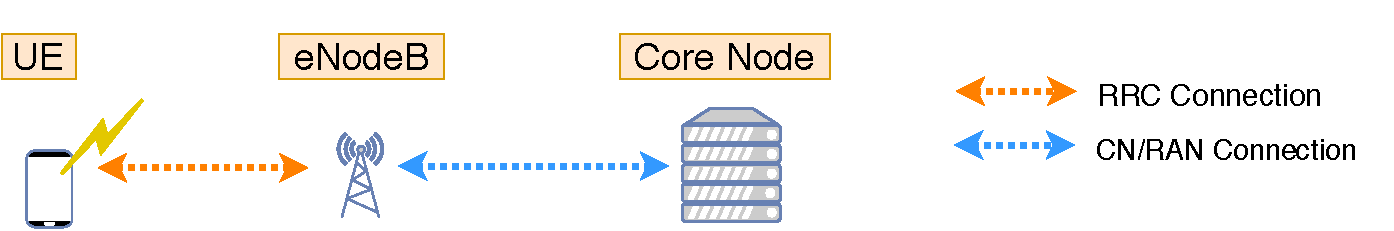
\includegraphics[width=0.7\hsize]{Connected.pdf}
  \caption{Connected}
	\label{Connected}
\end{figure}

\begin{figure}[htbp]
	\centering
	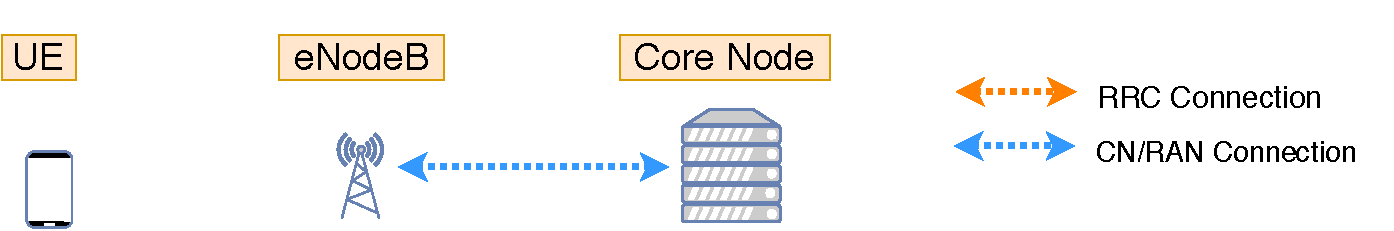
\includegraphics[width=0.7\hsize]{Connected_Inactive.pdf}
  \caption{Connected Inactive}
	\label{Connected Inactive}
\end{figure}

\begin{figure}[htbp]
	\centering
	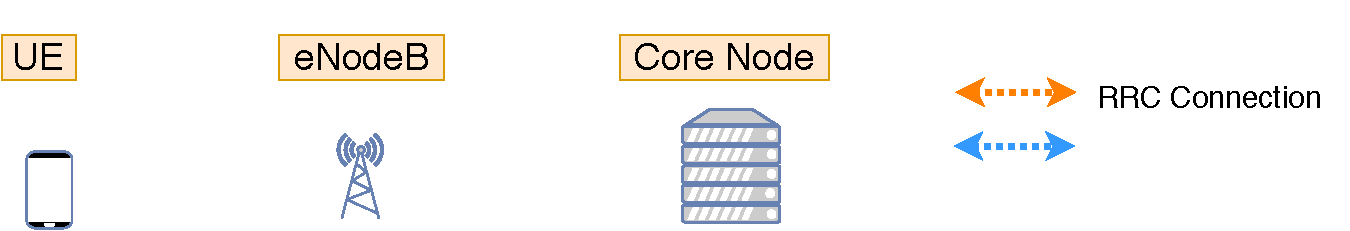
\includegraphics[width=0.7\hsize]{Idle.pdf}
  \caption{Idle}
	\label{Idle}
\end{figure}
\clearpage

上述のRRC Connected InactiveおよびRRC SuspendedをM2M/IoT端末に適応することは、CPUやメモリなどのサーバリソースの効率的な割り当てを難しくすると考えられる。
なぜなら、RRC Connected InactiveやRRC Suspendedはその特性から、端末がデータを送信していないタイミングにおいてもその端末情報をネットワークに保持するため、コアネットワークノードのメモリに対してこれまで以上の大きな負荷を発生させるためである。
また、M2M/IoT端末の接続台数の予測が難しいこともリソースの割り当てを難しくする一因である。
M2M/IoT端末は、スマートフォンのようなユーザ端末とは異なり、家電や自動車、電気メーター、センサなど様々な場所、様々な用途で使用される可能性があり、端末の台数およびその分布を予測することは困難であると考えられる。
このように、新たな状態の導入や、接続台数の予測が難しいIoT端末の普及により、今後のネットワーク事業者は、コアネットワークノードへのサーバリソースの割り当てがより難しいくなると予想される。

上述のようなネットワーク(サーバリソース消費の予測が難しく、変動が激しいネットワーク)において、収容可能な端末の増加を目的とした既存研究には、スケールアウトの考え方を用いたものが多い。
これらの研究では主に稼働するサーバやインスタンスの数をリソースの需要に応じて変動させることにより、ネットワークの変動に対応している。
しかし、この方法では、本来必要とされているリソース量(需用量)よりも多くのリソースが供給される、オーバープロビジョニングが発生する問題がある。
なぜなら、これらの研究では、サーバやインスタンス一台あたりのリソース量は一定であることを前提にした研究が多く、細かい粒度でリソースを制御できないためである。
また、必要とされるCPUとメモリのリソース比があらかじめ分かっていることを前提とした研究が多く、必要とされるリソース比が未知の場合はリソースの効率的な利用ができないからである。
例えば、CPUのリソース不足を解消するためにケールアウトを行った場合、CPUリソースと同時にメモリリソースも増加する。
しかし、メモリは元々ボトルネックにはなっていないため、新たに追加されたメモリはオーバープロビジョニングされたことになる。


このような背景から、CPUとメモリのリソース消費の予測が難しような状況や変動が大きいような状況においても、どちらかがボトルネックにならずに、効率的にリソースを活用するアーキテクチャを考えることは重要である。
実際、CPUとメモリのリソースを効率よく活用する研究は、データセンターなどの分野では行われている\cite{TechnoEconomicFrameworkforCloudInfrastructureACostStudyofResourceDisaggregation}。
しかし、モバイルネットワークに特化した研究は行われていない。
そこで、私はモバイルネットワークに特化した、CPUとメモリのリソースのオフロードを可能にする仕組みを考案する。
この方法により、CPUが過負荷である場合は、メモリの負荷を増加させる代わりにCPUの負荷を削減することが可能である。
またその逆に、メモリが過負荷である場合は、CPUの負荷を増加させることによりメモリの負荷を削減できる。
この仕組みにより、CPUとメモリのリソース消費の予測が難しい場合や、変動が激しいネットワークであっても、CPUおよびメモリ双方のリソース利用率の向上が期待でき、収容可能な端末の増加が期待できる。


% 私の案は、本来ならデタッチ処理が行われるタイミングであってもあえてデタッチ処理を行わないようにすることである。つまり、M2M/IoT端末がデータの送信を終え、電源をOFFにした後も、一部のセッションはそのまま維持しつつける。そして、M2M/IoT端末が再びONになりデータを送信する際には、以前と同じベアラを用いてデータを送信する。この方法によって、最初に一度アタッチ処理を行えば、その後のデータ送信においては、アタッチ処理は発生しないで済むため、アタッチおよびデタッチ処理を行うために必要なCPU負荷を削減しすることが可能である。
% 一方、本来は解放されるはずのセッション情報を維持し続けるため、その分メモリへの負荷が大きくなる。メモリのリソースが不足し、CPUリソースに余裕がある場合は、デタッチ処理が発生するまでの時間を短くすることにより、ベアラを維持するために必要なメモリリソースを積極的に解放してメモリ負荷を削減する。一方、その分デタッチ、アタッチ処理が頻繁に発生するため、CPUへの負荷は大きくなる。

% \subsection{負荷とそのオフロードの概要}
% \subsubsection{CPU負荷}
% CPU負荷は、主にアタッチやデタッチなどのシグナリング処理を各ノードで実行する際に発生する。時間当たりのシグナリング処理の実行回数の増加に伴い、負荷が増加する。CPU負荷の増加は、各ノードにおける処理時間の増大を引き起こす。また、CPUが過負荷状態になると、それ以上のシグナリング処理の実行が困難になる。
% \subsubsection{メモリ負荷}
% メモリ負荷は、主にベアラなどのセッションを維持するために必要な情報(ベアラ識別子、UE情報、ステート情報など)を保持する際に発生する。維持するベアラの増加に伴い、負荷が増加する。メモリが過負荷状態になると、新しくベアラを確立するために、古いベアラを解放する必要がある。
% \subsubsection{負荷のオフロード}
% 負荷のオフロードに関するイメージ図を図\ref{cpu}に示す。各図は端末台数とCPUおよびメモリリソースの使用率の関係をそれぞれ赤および青の線で示している。端末台数とは、システムが収容しているUEの数である。リソースの使用率とは、システムが利用できるリソースの最大値(物理的な性能の限界値や、事前にオペレータが設定した閾値などが想定される)に対して、UEを収容するために割り当てる必要のあるリソース量の割合である。一台あたりのUEを収容するために必要なリソース量の平均値はグラフの傾きに表れており、この値はUEの通信特性に応じて変化する。
%
% 図\ref{cpu}は、メモリリソースと比較してCPUリソースを大きく消費するような通信特性を持つUEを収容した場合のグラフである。図\ref{cpu}(a)を見ると、UE台数が$a$台の時点でCPU使用率が100\%に達していることがわかる。そのため、収容可能なUEの台数は$a$台である。一方、図\ref{cpu}(b)では、第\ref{sec:des}節で述べる方法により、一台あたりのUEを収容するために必要なリソース量を変化させた場合のモデルである。この図の例では、ボトルネックであったCPUの負荷をメモリにオフロードすることにより、収容可能なUE台数が$a$台から$a'$台に増加している。このように、CPUリソースが不足し、メモリリソースが余っているような場合においては、CPUの負荷をメモリにオフロードすることにより収容可能なUEの台数が増加する可能性がある。同様にCPUリソースが余っている状態で、メモリリソースが不足している場合においては、メモリからCPUへ負荷をオフロードすることが可能である。
%
% \begin{figure}[p]
% 	\centering
% 		\begin{subfigure}{1.0\textwidth}
% 			\centering
% 			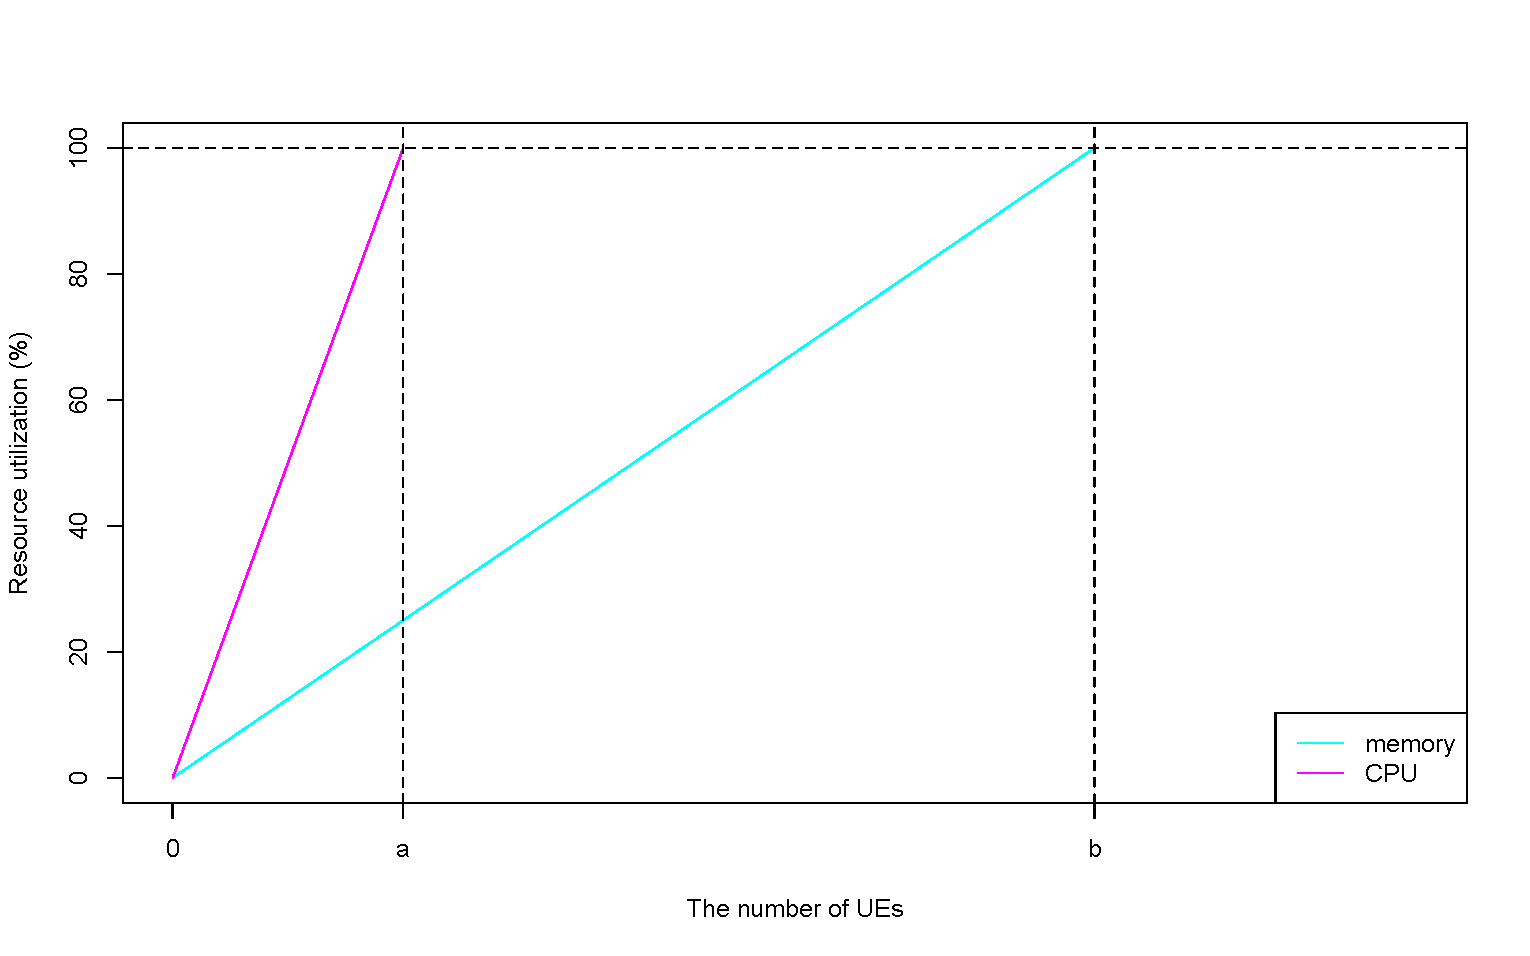
\includegraphics[width=1.0\hsize]{plot1.pdf}
% 			\caption{オフロードを行わない場合}
% 			\label{overcpu}
% 		\end{subfigure}
% 		\begin{subfigure}{1.0\textwidth}
% 			\centering
% 			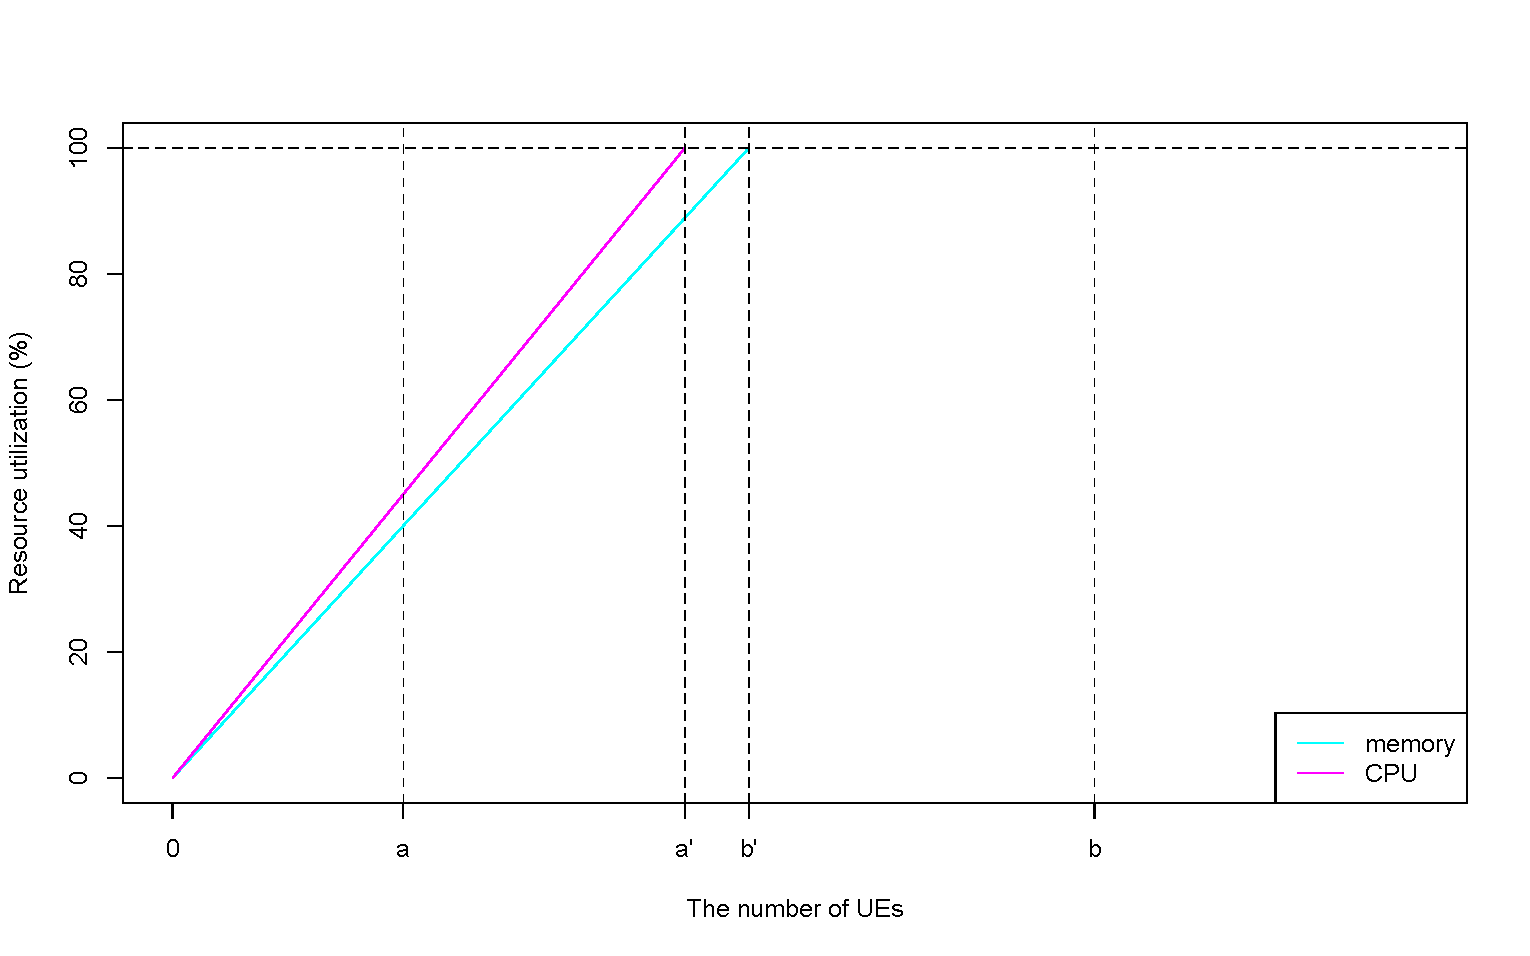
\includegraphics[width=1.0\hsize]{plot2.pdf}
% 		  \caption{オフロードを行った場合}
% 			\label{okcpu}
% 		\end{subfigure}
% 		\caption{CPU負荷をメモリへオフロード}
% 		\label{cpu}
% \end{figure}
% \clearpage

% \subsection{負荷のオフロード方法}
% \label{sec:des}
% Idle timer(UEがネットワークから切り離されたあと、デタッチ処理が行われるまでの時間)を$t$とする。通常、この時間は一定である。私は、$t$を変化させることによって、CPUとメモリの間で負荷をオフロードできるのではないかと考えた。
% 図\ref{detach-ON}は、M2M/IoT端末が最初にネットワークに接続した際の様子を示したものである。通常通り、アタッチの処理を行い、ベアラを確立する。図\ref{detach-OFF}は、M2M/IoT端末がネットワークから切断された際の様子である。通常は、数秒後にデタッチ処理が行われ、ベアラは全て解放されるが、$t$を長く設定した場合、デタッチ処理が行われないため、ベアラはそのまま維持される(UE-eNodeB間の無線帯域は解放する)。図\ref{detach-reON}はM2M/IoT端末が再びネットワークに接続した時の様子を示す。この場合、以前使用したベアラが残っているため、M2M/IoT端末は無線部分以外のアタッチ処理をスキップしてデータの送受信を開始できる。結果的に、EPCノードで行うアタッチ処理およびデタッチ処理の回数が削減されるため、CPUに与える負荷が削減される。一方、ネットワークに接続されていないM2M/IoT端末のセッション情報を保持する必要があるため、メモリが圧迫されることが予想される。
%
% Idle timer$t$を超えてもUEが再接続しない場合は、デタッチ処理を行う(図\ref{detach-timeout})。また、タイムアウト後に再接続する場合は、全てのベアラを新たに確立する必要がある(図\ref{detach-timeout-ON})。そのため、$t$を短く設定した場合は、デタッチ処理およびアタッチ処理が頻発するため、CPUの負荷が大きくなることが予想される。一方で、各ノードでセッション情報を保持する時間を短くすることができ、メモリの負荷の削減が期待できる。
%
%
%
% \begin{figure}[htbp]
% 	\centering
% 	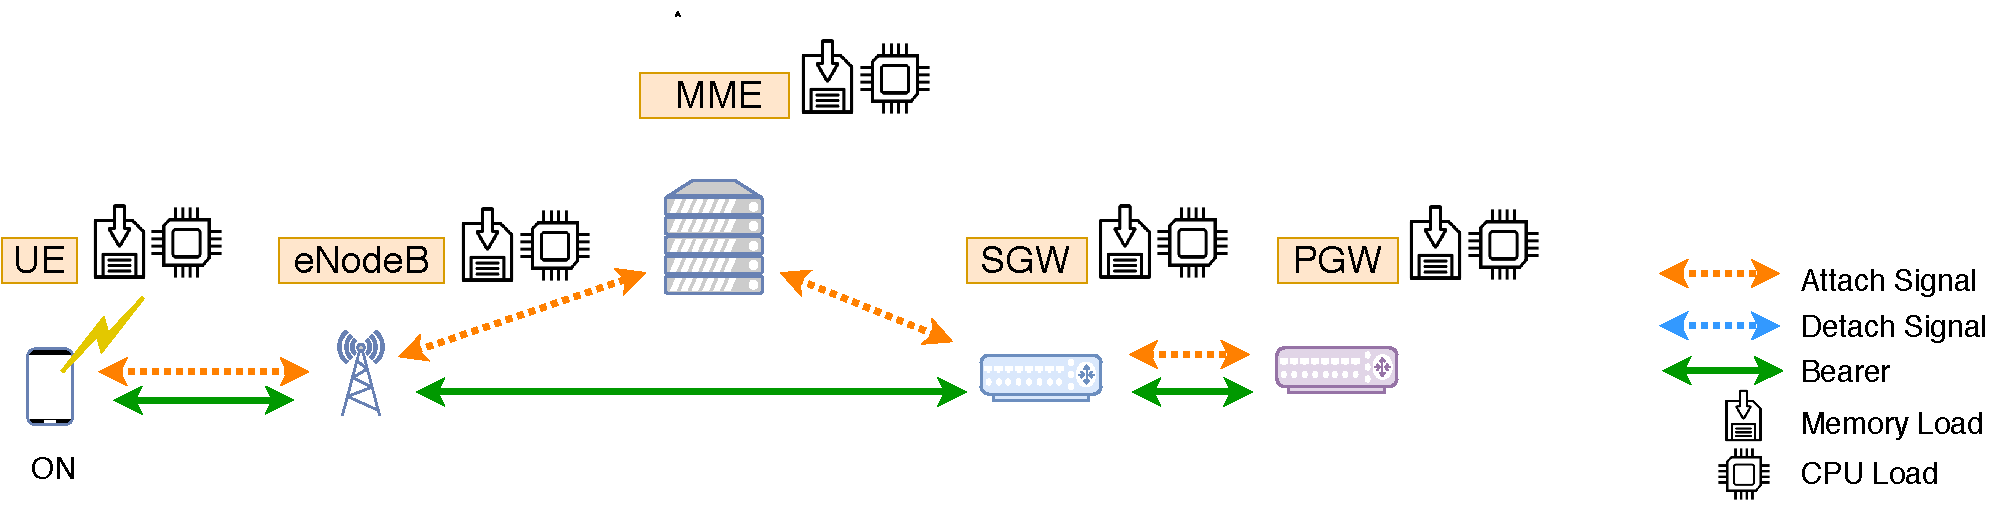
\includegraphics[width=0.7\hsize]{detach-ON.pdf}
%   \caption{UEが最初にネットワークに接続した時の処理}
% 	\label{detach-ON}
% \end{figure}
%
% \begin{figure}[htbp]
% 	\centering
% 	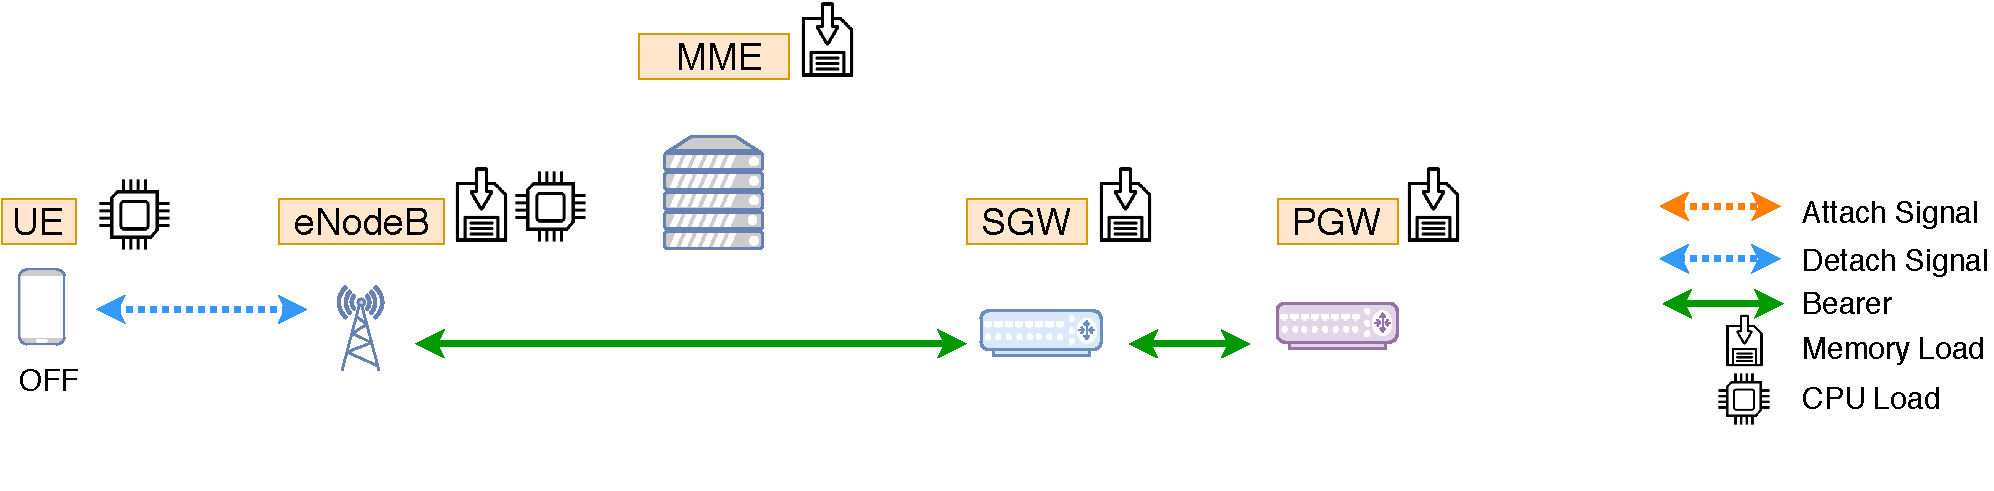
\includegraphics[width=0.7\hsize]{detach-OFF.pdf}
%   \caption{UEがネットワークから切り離された時の処理}
% 	\label{detach-OFF}
% \end{figure}
%
%
% \begin{figure}[htbp]
% 	\centering
% 	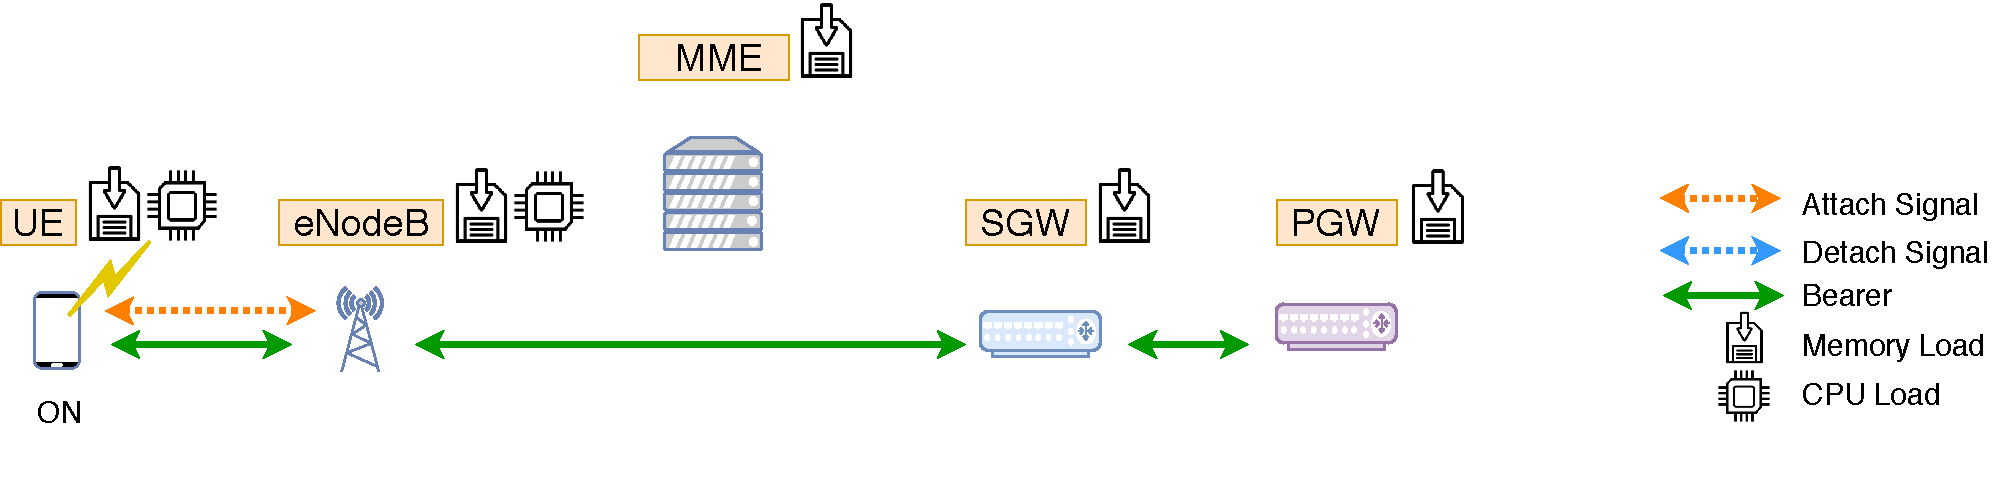
\includegraphics[width=0.7\hsize]{detach-reON.pdf}
%   \caption{ベアラのタイムアウト前にUEが再接続した時の処理}
% 	\label{detach-reON}
% \end{figure}
%
% \begin{figure}[htbp]
% 	\centering
% 	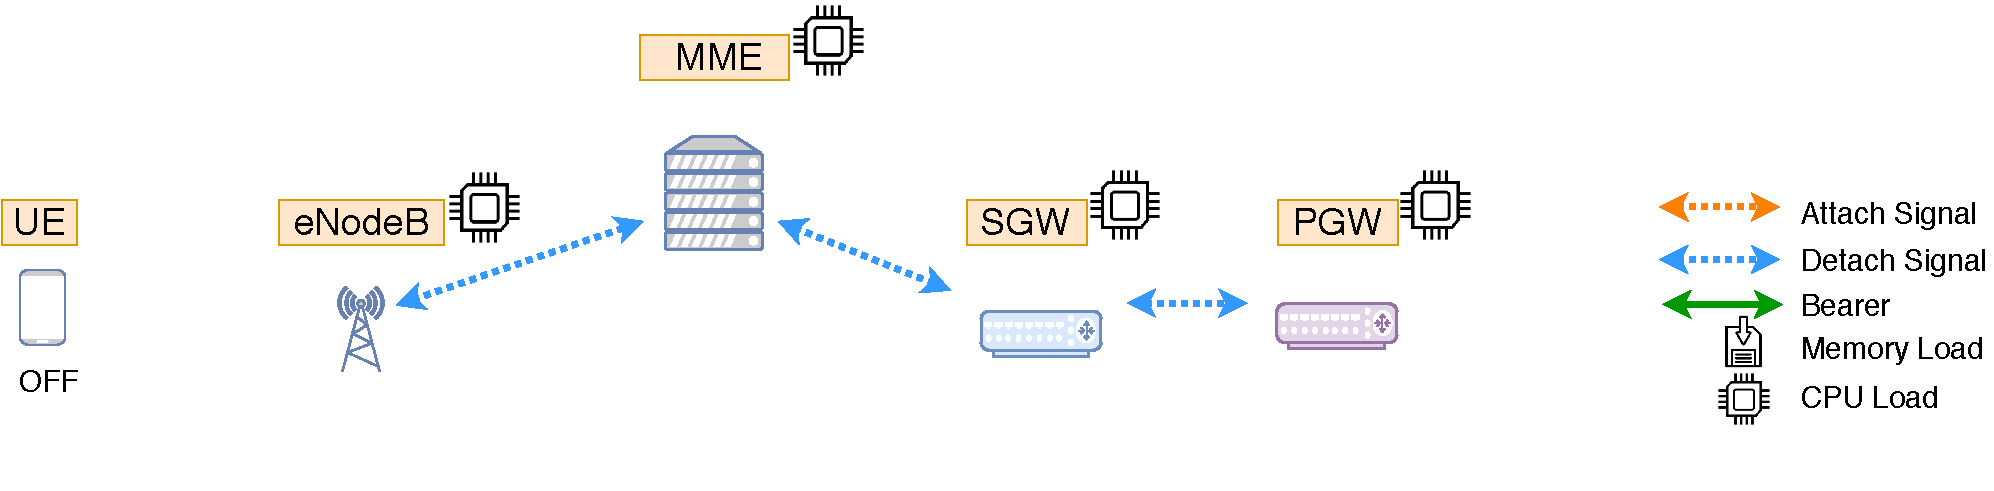
\includegraphics[width=0.7\hsize]{detach-timeout.pdf}
%   \caption{ベアラのタイムアウトが発生した場合の処理}
% 	\label{detach-timeout}
% \end{figure}
%
% \begin{figure}[htbp]
% 	\centering
% 	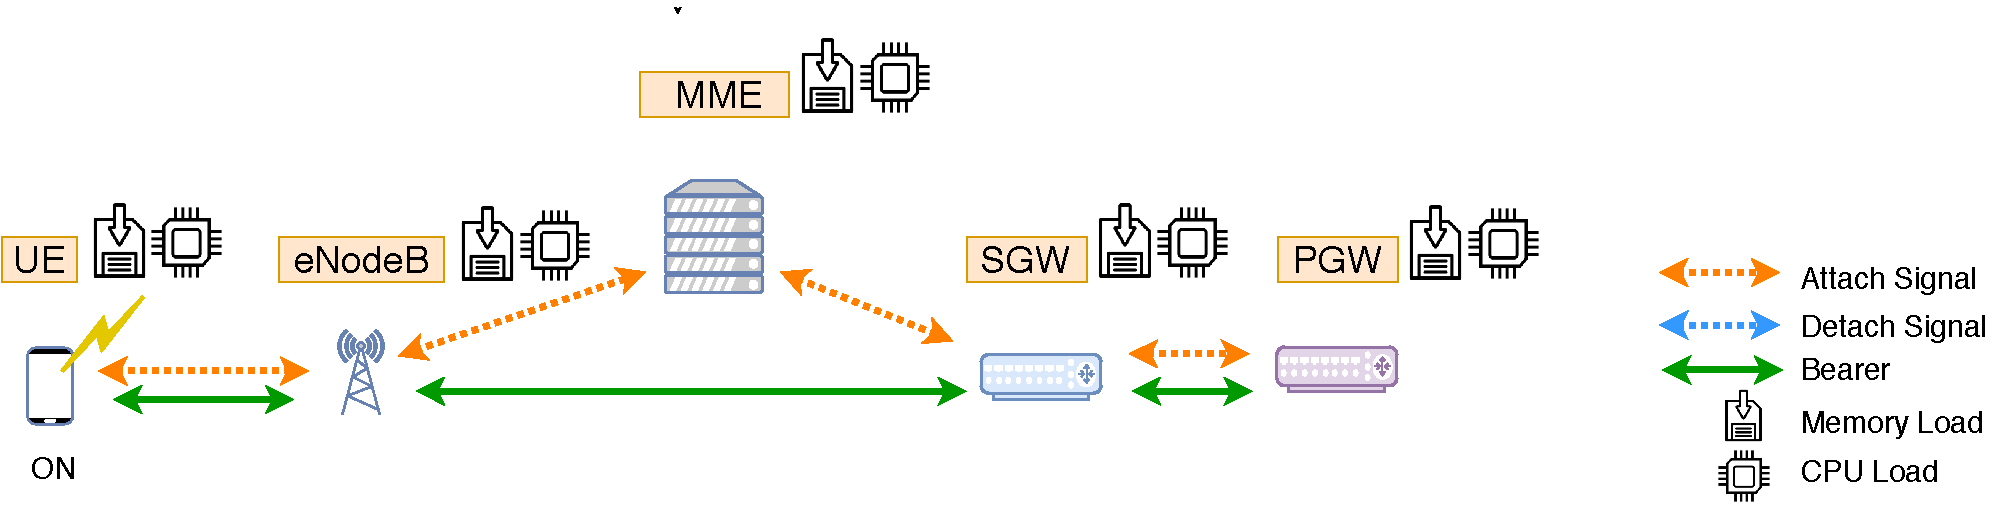
\includegraphics[width=0.7\hsize]{detach-timeout-ON.pdf}
%   \caption{ベアラのタイムアウト後にUEが再接続した場合の処理}
% 	\label{detach-timeout-ON}
% \end{figure}
%
% 前述のように、Idle timerを変更することにより、CPUとメモリの間で負荷をオフロードできると考えられる。これに実装した場合に想定される処理の流れを図\ref{chart}に示す。なお、第\ref{sec:method}節でのべる評価では、この処理を実行することおよび各ノードの負荷を監視することによる追加の負荷は発生しないと仮定している。
% \begin{figure}[htbp]
% 	\centering
% 	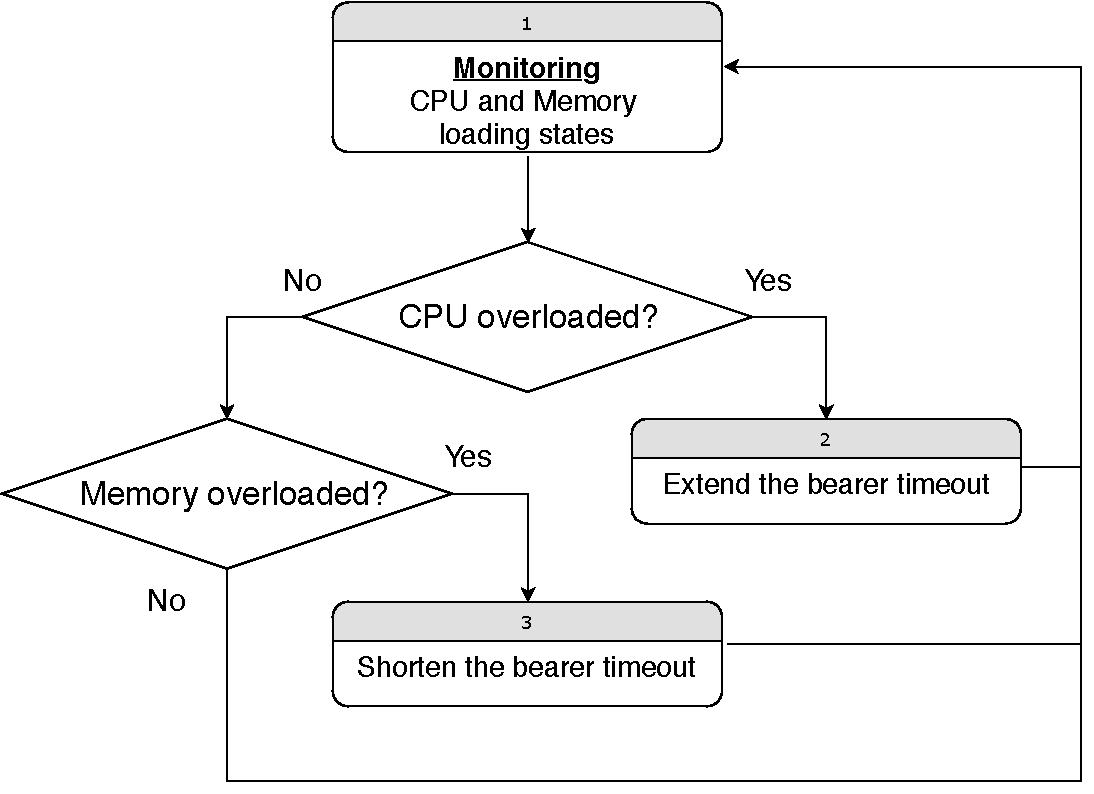
\includegraphics[width=0.7\hsize]{chart.pdf}
%   \caption{Idle timerの更新手順}
% 	\label{chart}
% \end{figure}












\clearpage
\section{提案手法}
また、UEが最後にデータ送信した後、Idle状態に遷移するまでの時間をIdle timerと定義する。
また、ネットワークが収容できる端末の最大数を、収容可能な端末台数と定義する。

本研究では、CPUとメモリのリソース利用率を最適化し、収容可能な端末台数を最大化するような、Idle timerの制御方法を提案する。
\subsection{Idle timerの設定}
提案手法では、Idle timerをCPUおよびメモリリソースの負荷状況に応じて動的に決定する。
Idle timerの設定によってコアノードのリソースの需要が変化する。提案手法では、ユーザ端末とM2M/IoT端末の存在割合に応じて、収容可能なUE台数を最大化するようなIdle timerを計算によって導出する。
処理のフローを図\ref{proposed_method}に示す。
常にCPUとメモリのリソース負荷を監視し、CPUが過負荷であればIdle timerを増加させ、反対にメモリが過負荷であればIdle timerを減少させる。
\begin{figure}[htbp]
	\centering
	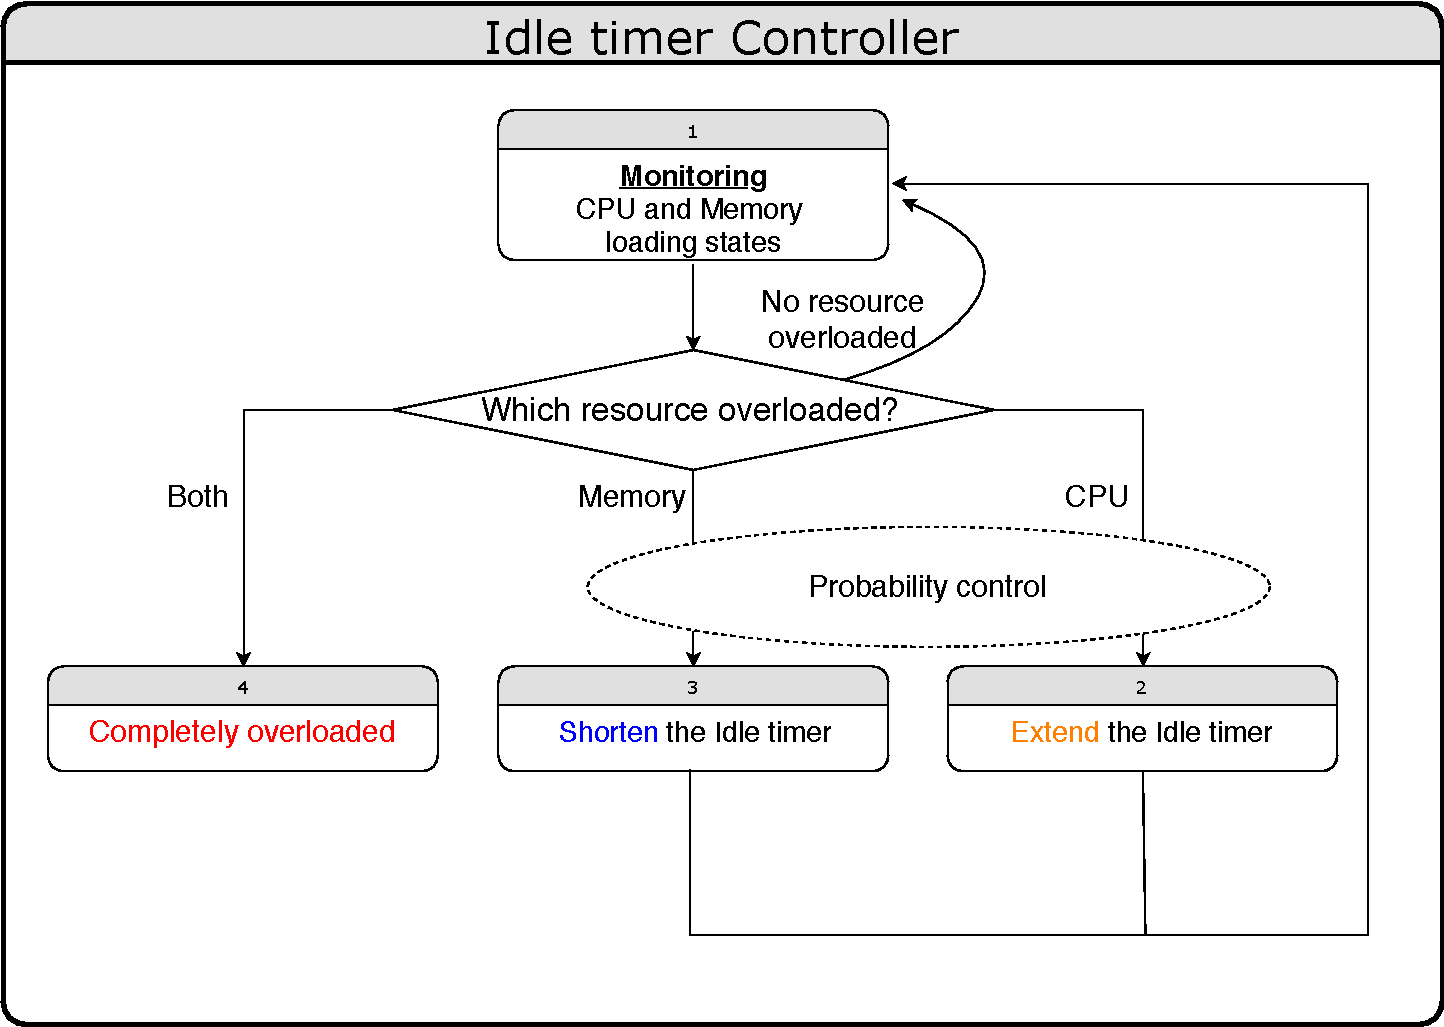
\includegraphics[width=0.7\hsize]{proposed_method.pdf}
  \caption{The proposed method}
	\label{proposed_method}
\end{figure}

% \subsection{Probability control}
% UEの通信特性が鋭いピークを持つ場合(特定の周期でデータ送信を行うUEが非常に多い場合)、Idle timerの設定が不安定になる可能性がある(\ref{spike})。
% そのため、場合によってはIdle timerの設定方法を拡張する必要がある。
% 具体的には、Idle timerに幅を持たせ、確率的にデタッチを実行する方法がある。
% \begin{figure}[htbp]
% 	\centering
% 	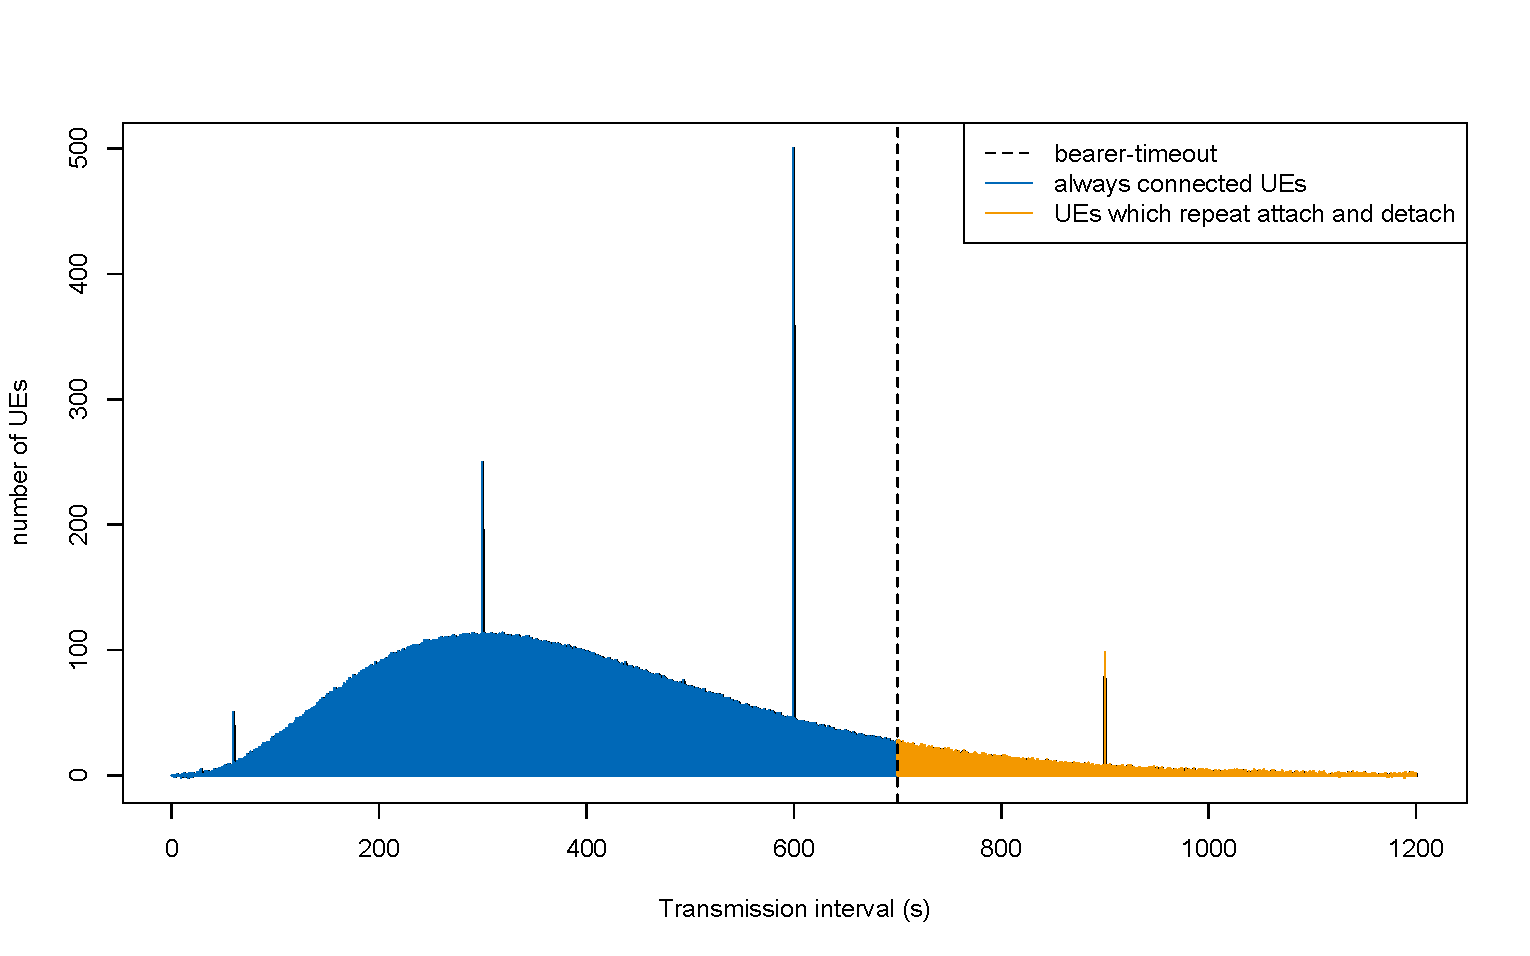
\includegraphics[width=0.8\hsize]{spike.pdf}
%   \caption{UEの通信特性が鋭いピークも持つ場合のイメージ}
% 	\label{spike}
% \end{figure}

\clearpage

\section{解析モデル}
\subsection{モバイルネットワーク}
単一のEPCで構成されるモバイルネットワークを対象として評価を行う。図\ref{networkmodel}に評価対象のネットワークを示す。図\ref{networkmodel}は以下のノードから構成される。
\begin{itemize}
  \item UE
  \item eNodeB
  \item MME
  \item S/PGW
\end{itemize}
UEおよびeNodeBは複数台、その他のノードは1台づつ存在する。
\begin{figure}[htbp]
	\centering
	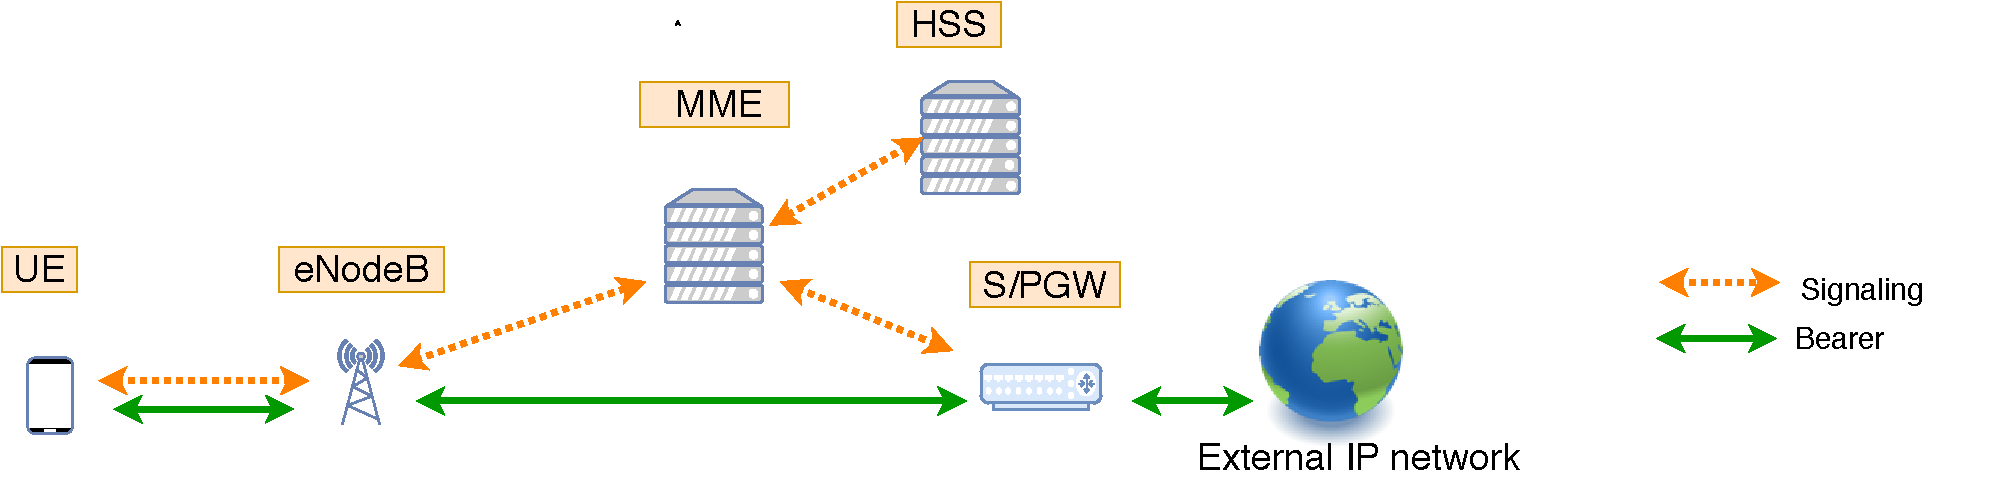
\includegraphics[width=0.7\hsize]{networkmodel.pdf}
  \caption{LTE/EPCネットワークモデル}
	\label{networkmodel}
\end{figure}

\subsection{状態遷移モデル}
UEが最後にデータを送信した後、Connected Inactive 状態に遷移するまでの時間を$T_{connect}$、Idle timerを$T_{timer}$と定義する。
あるUEにおけるデータの送信間隔を$T_h$と定義した時、このUEの状態遷移を図\ref{state_tran}に示す。
まず、UEはデータを送信すると、Connected状態へ遷移する。
データ送信後$T_{connect}$時間Connected状態を維持したのち、Connected Inactive状態へ遷移する。
そして、データ送信後$T_{timer}$後にIdle状態へ遷移する。
\begin{figure}[htbp]
	\centering
	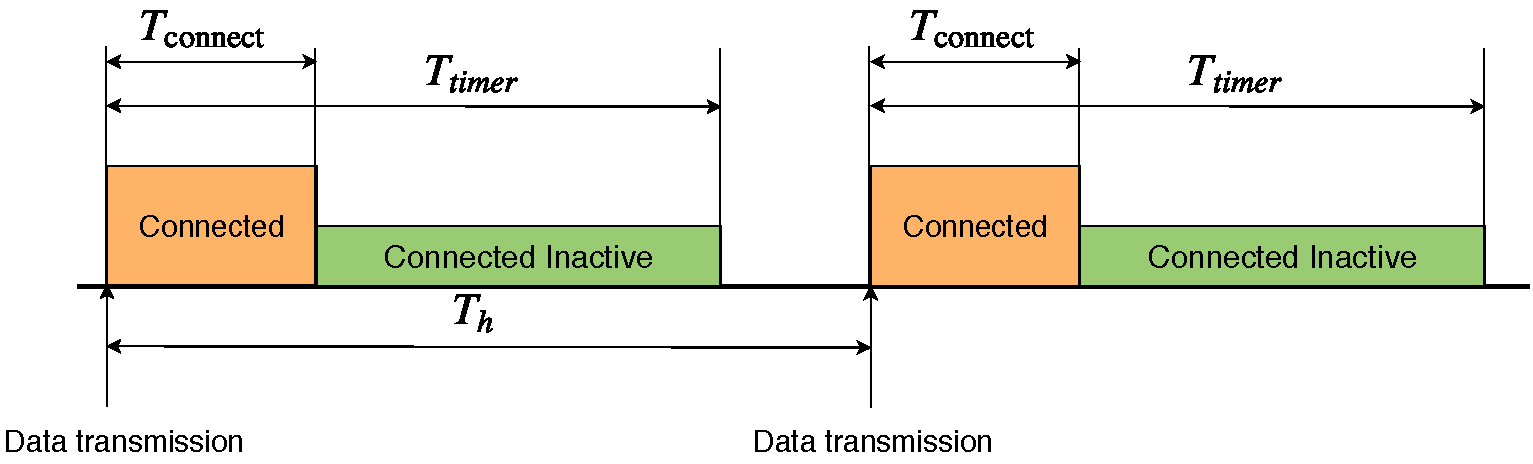
\includegraphics[width=1.0\hsize]{state_tran.pdf}
  \caption{状態遷移モデル}
	\label{state_tran}
\end{figure}

\subsection{UEの通信特性}
UEの通信特性はUEの種類によって異なる。例えばユーザ端末やM2M/IoT端末には以下のような特徴がある。
\begin{description}
  \item[ユーザ端末] 連続的なデータ通信を行う。通信データ量は多いが、常時ネットワークに接続した状態であるため、シグナリング処理の発生頻度が小さい。
  \item[M2M/IoT端末] 間欠的な通信を行う。データ送信の頻度は少ないが、データ送信の度にネットワークへの接続および切断を繰り返すため、シグナリング処理の発生頻度が大きい。また、データの送信周期に偏りがあると考えられる。
\end{description}
上述のようにUEの用途に応じて通信特性は変化する。そのため今回の評価では、ユーザ端末およびデータの送信間隔が異なる複数種類のIoT端末が存在することを想定して評価を行う。また、それぞれのUEの存在割合をパラメータとして変化させる。


\subsection{サーバ資源の割り当て}
今後検討予定である。


\subsection{解析環境}
\label{sec:method}
今回の研究はシミュレーションを用いてネットワークの性能評価を行う。
シミュレーションのタイムステップは1分から5分程度を想定している。
各タイムステップでは、UEの通信特性とIdle timerに基づきEPCの負荷を算出する。

EPCの負荷の算出のイメージ図を図\ref{analysis_environment}に示す。
UEの通信特性とIdle timerを入力とし、EPCの負荷を出力とする。
EPCのメモリ負荷の導出のために上野さんの実験結果を用いる。
\begin{figure}[htbp]
	\centering
	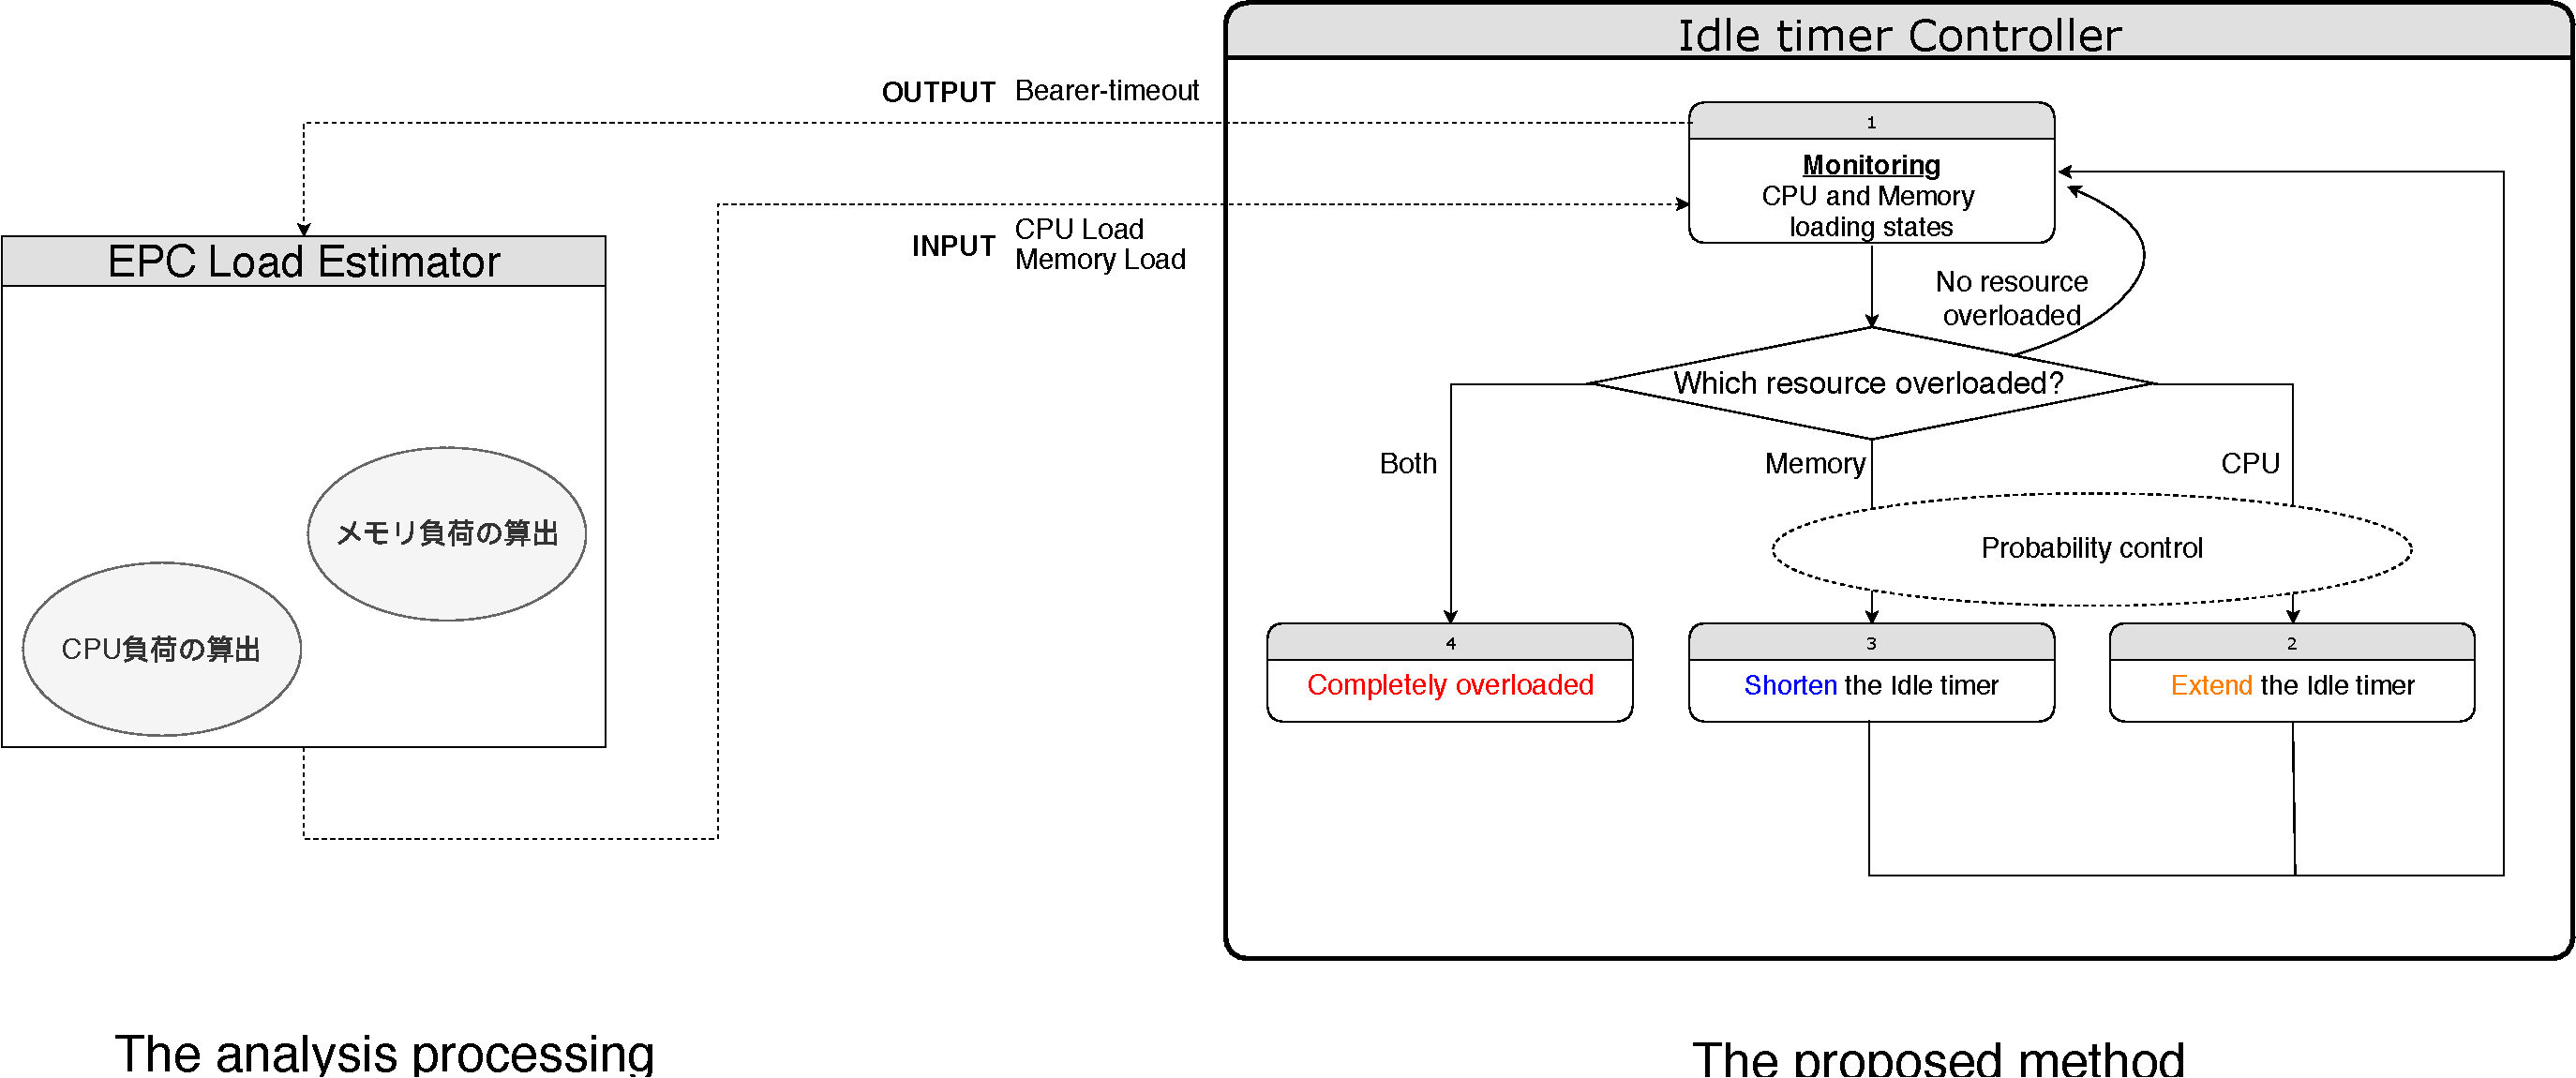
\includegraphics[width=0.9\hsize]{analysis_environment.pdf}
  \caption{解析環境}
	\label{analysis_environment}
\end{figure}
\clearpage

\subsubsection{統計処理}
この項では、UEの通信特性とIdle timerから、モバイルネットワークにおけるシグナリングの発生レートおよびベアラの平均接続数を導出する。

まず、ネットワーク全体におけるシグナリングの発生レートを求める。
$N_{UE}$台のUEがネットワークに存在すると仮定した時のUEの集合$\bm{U}$を、$\bm{U} = \left\{ u_1,u_2,\ldots,u_{N_{UE}} \right\}$と定義する。
あるUE $u_h$ $(u_h \in \bm{U})$が1秒あたりに発生させるシグナリングの数を$s_h$と定義する。
最後のデータ送信からConnected Inactive状態へ遷移するまでの時間を$T_{connect}$、Idle timerを$T_{timer}$、$u_h$の通信周期を$T_h$とする。
また、状態遷移に伴うシグナリングの発生回数をそれぞれ表\ref{table:state}のように定義すると、$s_h$は以下の式(\ref{eq:attach_detach})で表せる。
ここで留意すべきは、$T_h$が$T_{connect}$以下であるようなUEは、一度Connected状態に遷移すると、常時Connected状態を維持し、状態遷移によるシグナリングが発生しないため、$s_h$は0と定義したことである。
\begin{table}[h]
 \caption{state signaling}
 \label{table:state}
 \centering
  \begin{tabular}{ccc}
   \hline
   Source & Destination & The number of signaling occurrences \\
   \hline \hline
   Connected & Connected Inactive & $n_{connect \to inactive}$ \\
   Connected Inactive & Connected & $n_{inactive \to connect}$ \\
   Connected Inactive & Idle & $n_{inactive \to idle}$ \\
   Idle & Connected  & $n_{idle \to connect}$ \\
   \hline
  \end{tabular}
\end{table}

\begin{equation}
  s_h  =
  \begin{cases}
		0 & \text{if $T_h \le T_{connect}$} \\
    \frac{1}{T_h} \cdot (n_{inactive \to connect} + n_{connect \to inactive}) & \text{if $T_{connect} \le T_h \le T_{timer}$} \\
    \frac{1}{T_h} \cdot (n_{idle \to connect} + n_{connect \to inactive} + n_{inactive \to idle}) & \text{otherwise}
  \end{cases}
  \label{eq:attach_detach}
\end{equation}

1秒毎にネットワーク全体で発生するシグナリングの合計を$S$と定義する。$S$は$s_h$を用いて以下の式(\ref{eq:all_signal})で表せる。
\begin{eqnarray}
  S & = & \sum_{h = 1}^{N_{UE}} s_h \label{eq:all_signal}
\end{eqnarray}

次に、各状態ごとのUE数を求める。
ある時刻において、UE $u_h$がConnected状態である確率を$b_{connected}$、Connected Inactive状態である確率を$b_{inactive}$、Idle状態である確率を$b_{idle}$と定義する。するとこれらの値は、$T_h$および$T_{timer}$、$T_{connect}$を用いて以下の式(\ref{eq:connected})、(\ref{eq:inactive})、(\ref{eq:idle})で表せる。
% ここでは、$s_h$が$T_{timer}$以下であるようなUEは、常時接続状態となるため、$s_h$は1と定義した。
\begin{align}
	b_{connected} & =
	\begin{cases}
    1 \hphantom{100000000000000} & \text{if $T_h \le T_{connect}$}\\
    \frac{T_{connect}}{T_h} & \text{otherwise}
  \end{cases} \label{eq:connected}\\
	b_{inactive} & =
  \begin{cases}
    0 \hphantom{100000000000000} & \text{if $T_h \le T_{connect}$}\\
		\frac{T_h - T_{connect}}{T_h} & \text{if $T_{connect} \le T_h \le T_{timer}$}\\
    \frac{T_{timer}}{T_h} & \text{otherwise}
  \end{cases} \label{eq:inactive}\\
	b_{idle} & =
  \begin{cases}
    0 \hphantom{100000000000000} & \text{if $T_h \le T_{connect}$}\\
		0 & \text{if $T_{connect} \le T_h \le T_{timer}$}\\
    \frac{T_h - T_{timer}}{T_h} & \text{otherwise}
  \end{cases}\label{eq:idle}
\end{align}

Conneted状態であるUEの平均数およびConnected Inactive状態であるUEの平均数、Idle状態であるUEの平均数を$B_{connected}$、$B_{inactive}$、$B_{idle}$と定義すと、それらは、は$b_{connected}$および$b_{inactive}$、$b_{idle}$を用いて以下の式(\ref{eq:connected_average})、(\ref{eq:inactive_average})、(\ref{eq:idle_average})で表せる。
\begin{eqnarray}
  B_{connected} & = & \sum_{h = 1}^{N_{UE}} b_{connected} \label{eq:connected_average}\\
	B_{inactive} & = & \sum_{h = 1}^{N_{UE}} b_{inactive} \label{eq:inactive_average}\\
	B_{idle} & = & \sum_{h = 1}^{N_{UE}} b_{idle} \label{eq:idle_average}
\end{eqnarray}


\subsubsection{シグナリング負荷に基づく評価}
\label{sec:cpu}
ネットワーク全体におけるシグナリングの発生レートから、CPUにかかる負荷を算出する。

\subsubsection{上野さんの実験に基づく評価}
\label{sec:memory}
上野さんの実験データを基にメモリ負荷を導出する。
図\ref{mme_memory}、図\ref{spgw_memory}、図\ref{hss_memory}に示す実験データから、ベアラの確立がEPCの各ノード(MME、SPGW、HSS)のメモリに与える影響を測定した。
その結果、UE1台あたりのベアラの確立がメモリに与える負荷はMME、SPGW、HSSでそれぞれ750KB、350KB、6KBであることが分かった。
この結果を参考にしてメモリ負荷を算出することを考えている。

\begin{figure}[htbp]
	\centering
	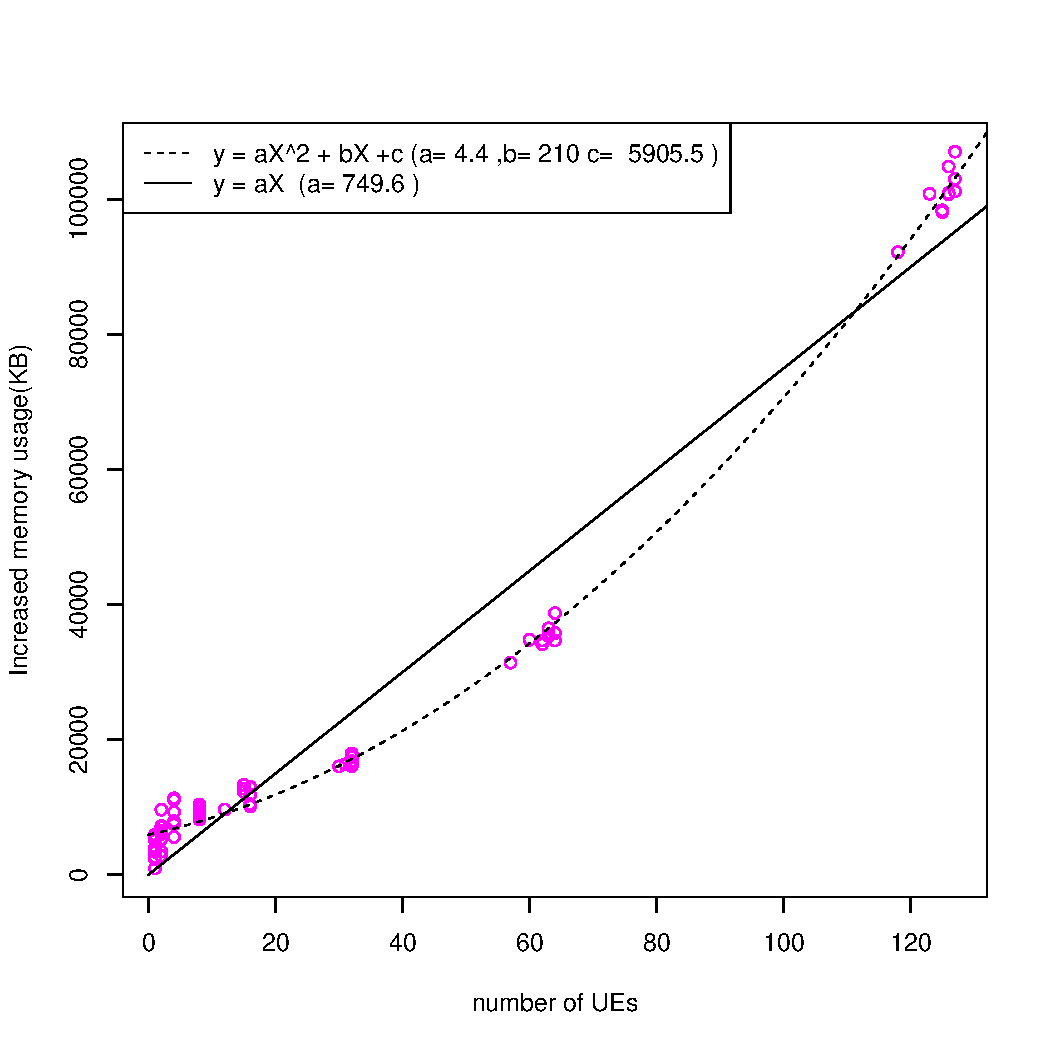
\includegraphics[width=0.7\hsize]{mme_memory.pdf}
  \caption{ベアラの確立によって増加したメモリ使用量(MME)}
	\label{mme_memory}
\end{figure}

\begin{figure}[htbp]
	\centering
	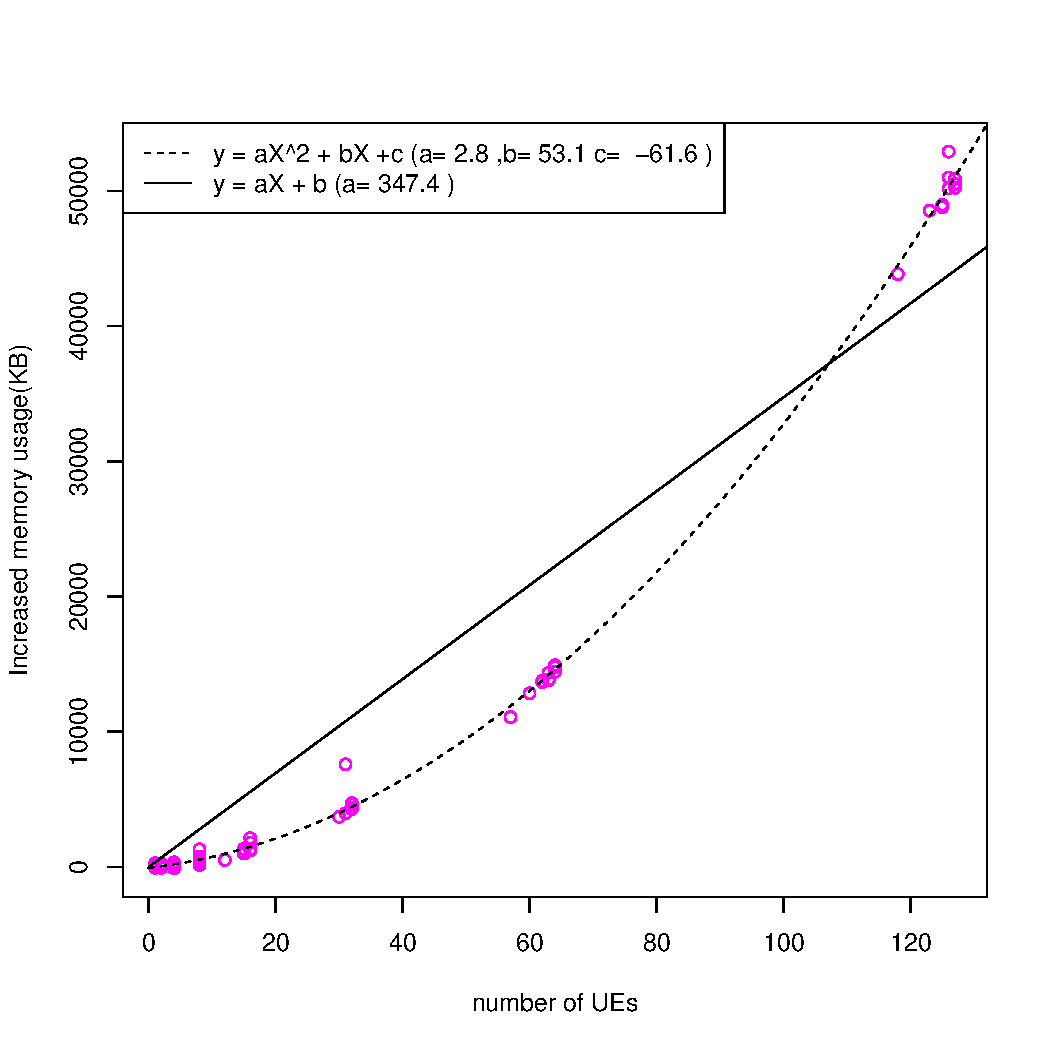
\includegraphics[width=0.7\hsize]{spgw_memory.pdf}
  \caption{ベアラの確立によって増加したメモリ使用量(SPGW)}
	\label{spgw_memory}
\end{figure}

\begin{figure}[htbp]
	\centering
	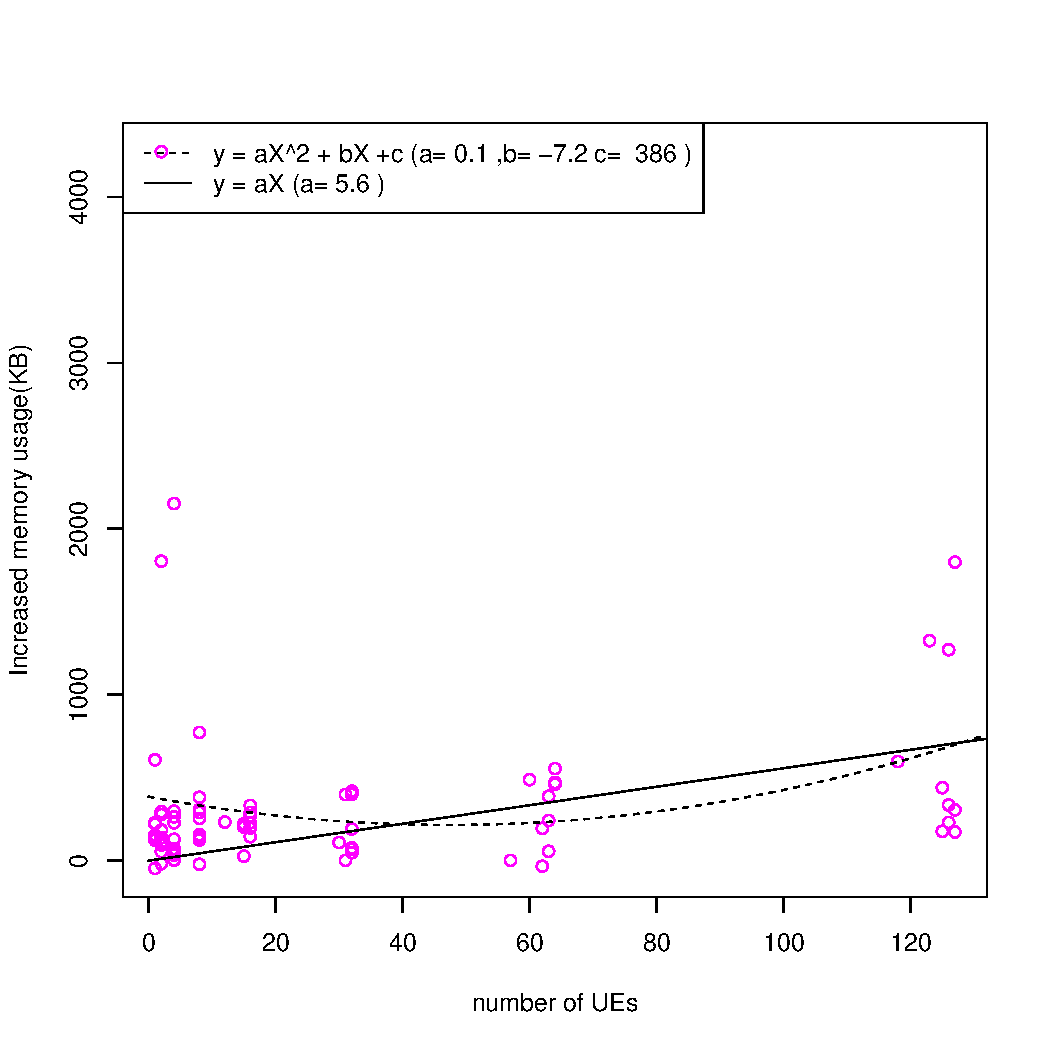
\includegraphics[width=0.7\hsize]{hss_memory.pdf}
  \caption{ベアラの確立によって増加したメモリ使用量(HSS)}
	\label{hss_memory}
\end{figure}
\clearpage



\section{先行研究調査}
サーバのリソース分離に関する文献\cite{TechnoEconomicFrameworkforCloudInfrastructureACostStudyofResourceDisaggregation}を調査した。この文献では、データセンタのコストを削減することを目的し、サーバリソースの分離を提案している。そして、サーバごとにリソース構成が固定されている従来のデータセンタと、CPUとメモリのリソース構成をサーバから分離したデータセンタとの比較を行っている。
評価の結果、リソースを分離することによって、CPUとメモリのオーバープロビジョニングを削減できることを示している。そして、コスト面では(アプリケーションにも依存するが)最大40\%の削減が期待でいると結論づけてる。

文献\cite{ModelingDelayTimerAlgorithmforHandoverReductioninHeterogeneousRadioAccessNetworks}では、モバイルネットワークにおいてハンドオーバに関わるシグナリングの発生回数を減らすことを目的とし、Delay Time Algorithem を提案している。このアルゴリズムでは、従来の仕組みであればハンドオーバ処理を行うような状況であっても、あえてハンドオーバ処理を行うタイミングを遅らせることによって、シグナリングの発生を削減することを可能としている。

文献\cite{ModelingofMobilityAwareRRCStateTransitionforEnergyConstrainedSignalingReduction}では、UEがCennected 状態から idel状態へ遷移するまでの時間(inactive timer)を制御することによって、シグナリング発生回数とUEの消費電力を最適化する研究を行っている。inactive timerを大きくすることによって、UEの状態遷移に伴うシグナリングの発生回数を抑えることが可能である一方、UEが長い時間Connected状態に止まるために消費電力が増加することを明らかにしている。

文献\cite{RRCStateHandlingfor5G}では、RRC Connected Inactive stateと呼ばれる状態を新しく導入することによって、シグナリングの発生回数及びUEの消費電力を削減できることを示している。


\section{今後の課題}
\begin{itemize}
  \item デタッチの処理負荷を求めるため、OAIに基づくデタッチ処理のプログラム行数を調査する。
  \item UEの通信特性の分布を決定する上で、根拠となるデータを見つける。
  \item メモリの負荷が二次関数的な増加を示している理由を調査する。調査方法としては、UE数およびeNodeB数のどちらか一方を固定し、もう一方を変化させつつベアラ確立の実験を行い、メモリ負荷を観測する。もしくは、OAIのソースコードを読みデータの保持に関する実装を調査する。
\end{itemize}
\section*{\addcontentsline{toc}{section}{参考文献}}
\bibliographystyle{IEEEtran}
\bibliography{/Users/t-adachi/Documents/study/Bibliography/bib/hpt_core_network/myBib/LABbiblio,/Users/t-adachi/Documents/study/Bibliography/bib/hpt_core_network/Study_Group_Bibtex/bib/hptCoreNetwork_Study}
\end{document}
